%
%  untitled
%
%  Created by Asger Pedersen on 2012-01-04.
%  Copyright (c) 2012 . All rights reserved.
%
\documentclass[]{article}

% Use utf-8 encoding for foreign characters
\usepackage[utf8]{inputenc}

% Setup for fullpage use
\usepackage{fullpage}

\usepackage{pdfpages}
% Uncomment some of the following if you use the features
%
% Running Headers and footers
%\usepackage{fancyhdr}

% Multipart figures
%\usepackage{subfigure}

% More symbols
%\usepackage{amsmath}
\usepackage{amssymb}
%\usepackage{latexsym}

% Surround parts of graphics with box
\usepackage{boxedminipage}

% Package for including code in the document
\usepackage{listings}

% If you want to generate a toc for each chapter (use with book)
\usepackage{minitoc}

% This is now the recommended way for checking for PDFLaTeX:
\usepackage{ifpdf}

%\newif\ifpdf
%\ifx\pdfoutput\undefined
%\pdffalse % we are not running PDFLaTeX
%\else
%\pdfoutput=1 % we are running PDFLaTeX
%\pdftrue
%\fi

\usepackage{ifpdf}
\title{ Project Course: Development Studio \\ Deliverable 4: Sprint \#3}
\author{ Asger Pedersen, Kristoffer Cobley, Hari Charan \& Jesper Tved }
\setlength{\parindent}{0pt}
\setlength{\parskip}{2ex}
\linespread{1.3}

\begin{document}

\ifpdf
\DeclareGraphicsExtensions{.pdf, .jpg, .tif}
\else
\DeclareGraphicsExtensions{.eps, .jpg}
\fi

\maketitle
\setcounter{tocdepth}{1}
\tableofcontents
\newpage
\section{Sprint Material} % (fold)
\label{sec:Sprint Material}
\subsection{Version} % (fold)
\label{sub:Version}
The current state of our app has version 0.0.1. Meaning that the app is still alpha quality, with some functionality implementet, but lot of unfinished work.
% subsection Version (end)
\subsection{Source code} % (fold)
\label{sub:Source code}
We still use Git and GitHub. The source code is available at: \verb!https://github.com/mundane/ETA_analytics!, in the app folder. The other folders contains prototypes and experiments.
% subsection Source code (end)
\subsection{Sprint Explanation}
The burndown chart shows that, in spite of exams and easter holidays stalled the progress of development in the beginning of the sprint, we did manage to finish some of the tasks within the sprint time frame.
\begin{figure}[h!]
  \centering
    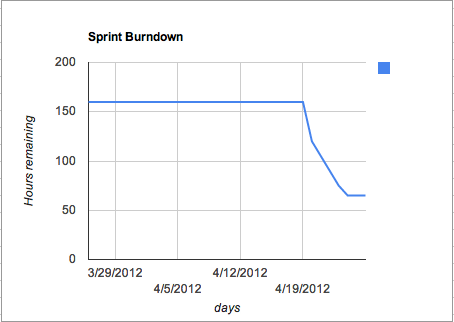
\includegraphics[width=0.8\textwidth]{images/burndown.png}
	\caption{Burndown chart for sprint \# 2. Easter holidays and exams is the reason for the steep curve.}
\end{figure}

\subsection{User Stories}
For sprint \# 2 we had the following user stories: \\
As an analytic \\
I want to make pie charts, column charts, bar charts, etc \\
So that I can make data more presentable \\

As an analytic \\
I want to make charts interactive  \\
So that I can make data more presentable \\

As an analytic \\
I want a way to show selected data from the chart \\
So that I can make data more presentable\\

As an analytic \\
I want to save data for later sessions \\
So I can continue working on datasets \\

\subsection{Tasks} % (fold)
\label{sub:Tasks}
We divided the stories up in the following tasks
% subsection Tasks (end)Tasks
\begin{itemize}
	\item Read up on the MVC model
	\item Research testing tools for Sencha
	\item Research JSLint
	\item Convert CSV format to JSON
	\item Create datagrid from JSON
	\item Make integration to Jstat in the datagrid view
	\item Create charts
\end{itemize}










% section Sprint Material (end)


\section{Sprint Retrospective} % (fold)
\label{sec:Sprint Retrospective}

% section Sprint Retrospective (end)

\section{Learning Goals} % (fold)
\label{sec:Learning Goals}

% section Learning Goals (end)
\section{Architectural Description} % (fold)
\label{sec:Architectural Description}

In the following we will be describing the current software architecture for our system. An architectural description could be used as a basis for stakeholder communication, as part of an on-going software design process or to evaluate different architectures \cite{christensen}. In the following we will be using the recommendations found in \cite{christensen} to describe the software architecture. In particular we will be using different viewpoints to communicate the overall structure of the system. In the following we will be looking at the model, C\&C view respectively, we will not be looking at the deployment view in our case, as our system is simple enough that this view would not add much to an overview.

\subsection{Model View}



\subsection{C\&C View}


% section Architectural Description (end)
\section{Documentation} % (fold)
\label{sec:Documentation}
Chosing to build our application in JavaScript means that finding a documenting tool was not particular easy, as tools like JavaDoc and doxygen are not applicable to JavaScript. In our research we happened upon JSdoc, \url{http://code.google.com/p/jsdoc-toolkit}
% section Entity Documentation (end)
\appendix
\section{Scrum Material} % (fold)
\label{sec:Scrum Material}

% section Scrum Material (end)
%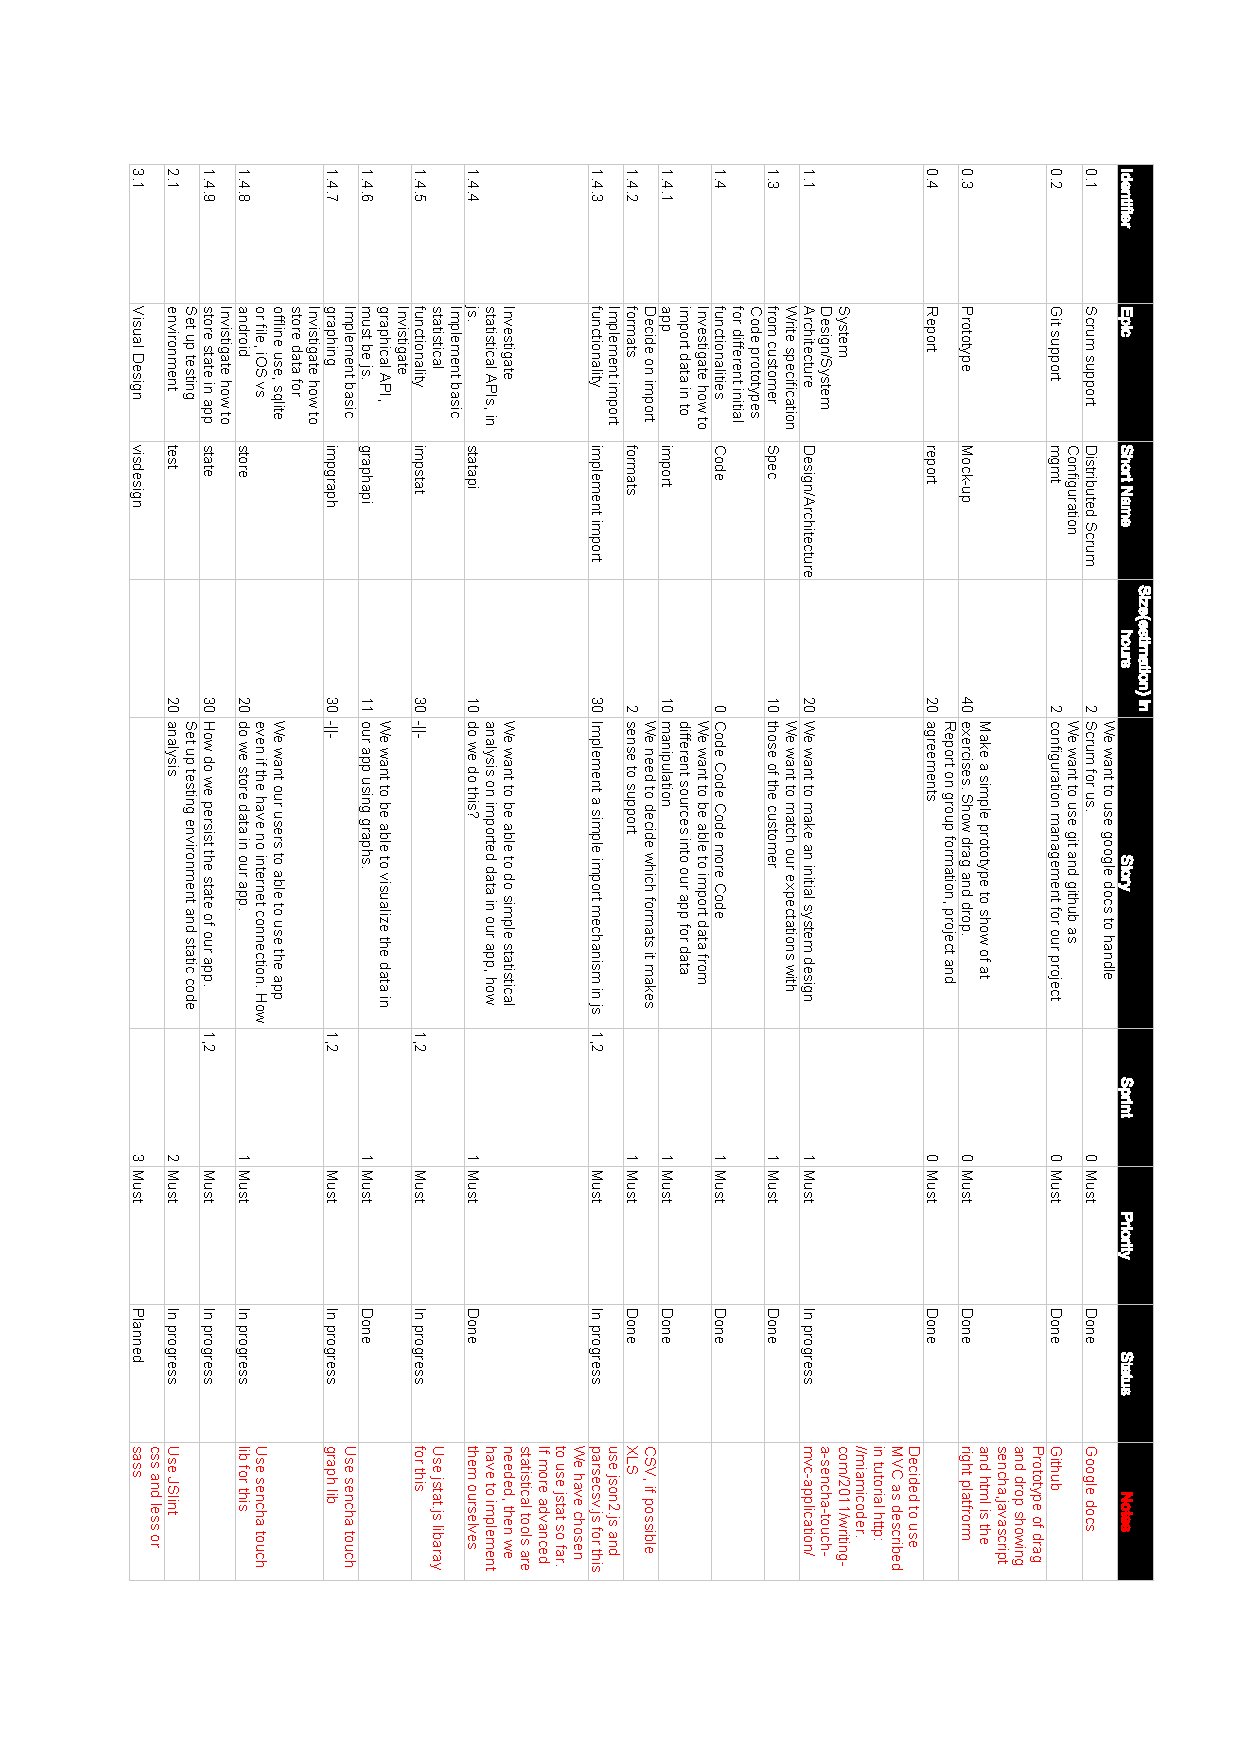
\includepdf[pages={-}]{images/backlog1.pdf}
%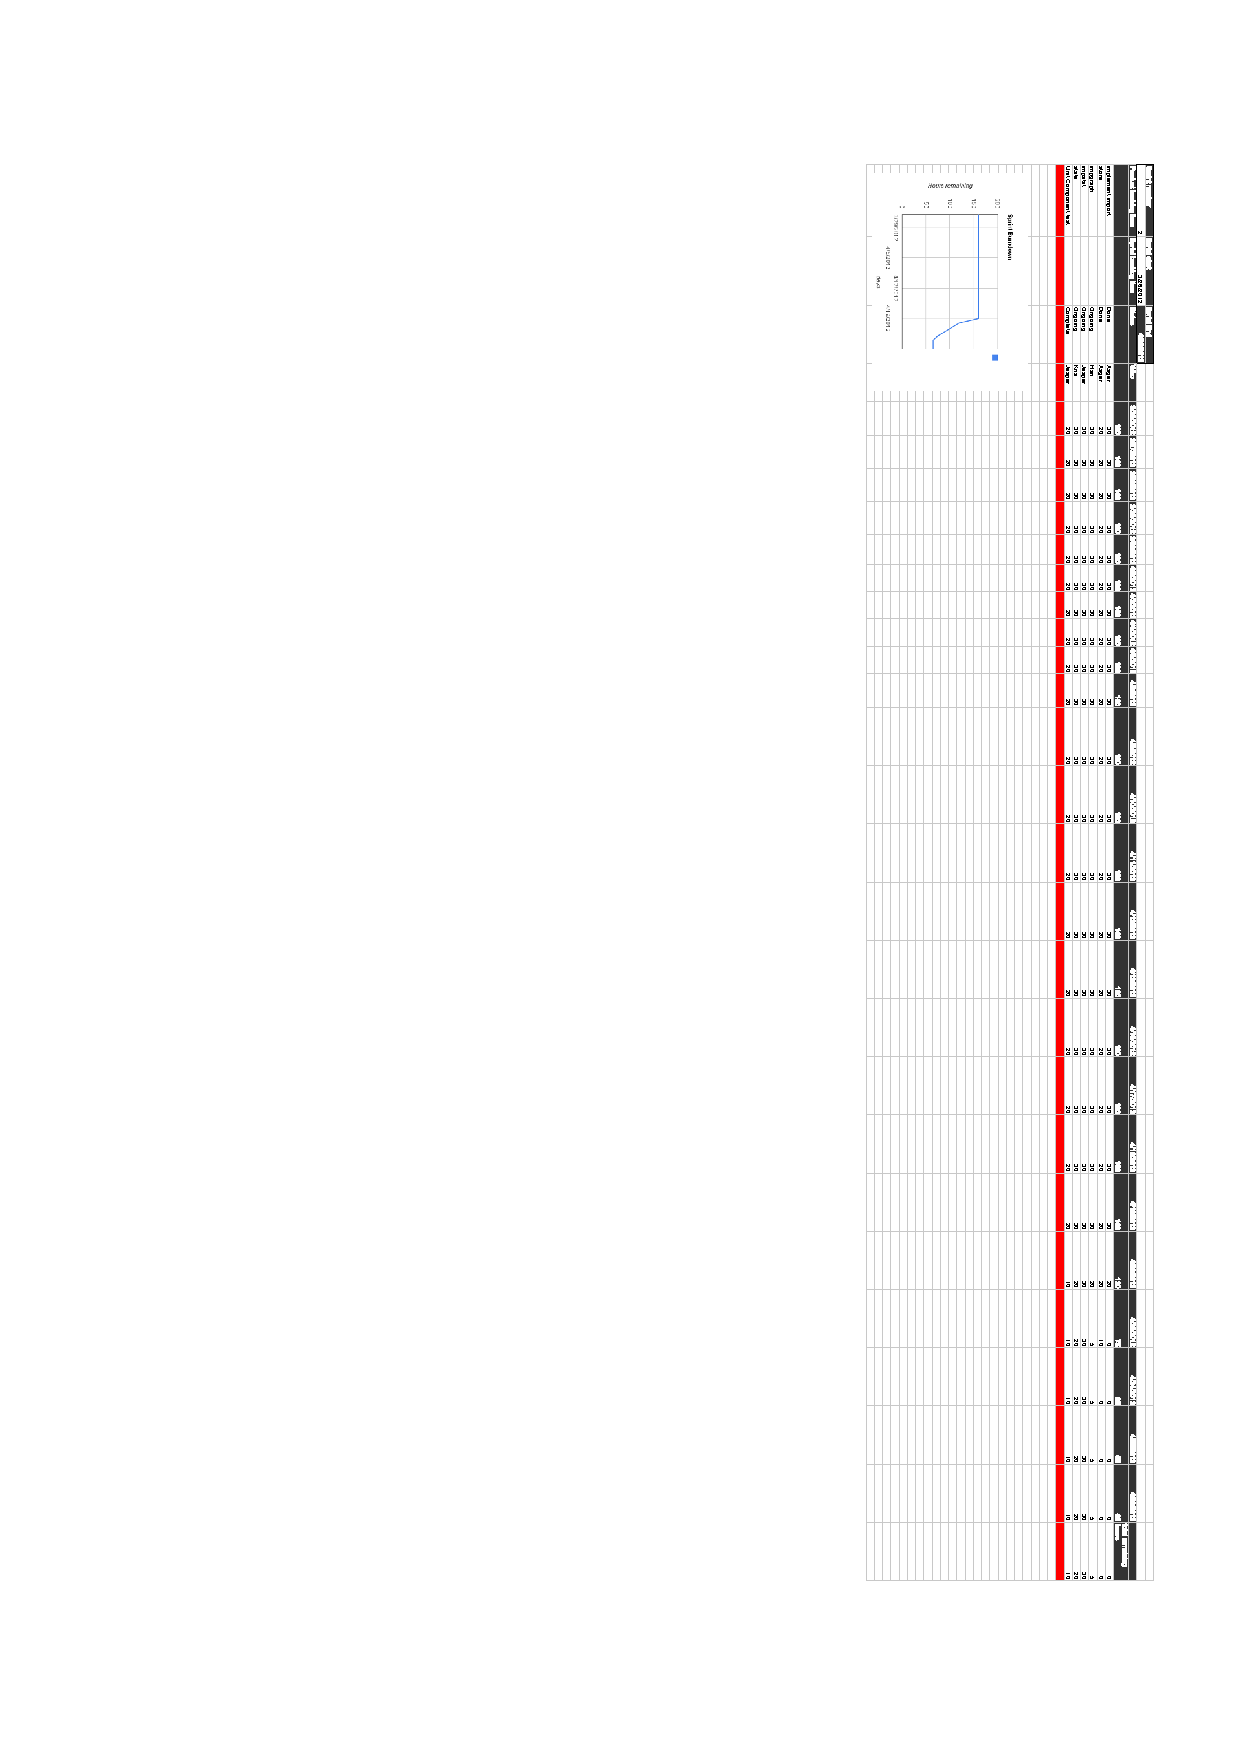
\includepdf[pages={-}]{images/sprint1.pdf}

\bibliographystyle{plain}
\bibliography{}
\end{document}